\begin{flushleft}
	\section{\textcolor{cyan}{Présentation du l’organisme d’accueil et le service accueillant : }}
	\subsection{\textcolor{green}{MolbiolExpert :}}

	MolbiolExpert est une entreprise spécialisée dans le domaine de la biologie et offre une gamme complète de services de pointe dans le domaine du diagnostic moléculaire, des puces à ADN, du séquençage haut débit, de la chimie, de l'immunoanalyse et de l'anatomie pathologique. Selon le responsable de MolbiolExpert, l'entreprise a été créée dans le but de s'épanouir dans le domaine du vivant et d'étendre son expertise à tous les aspects de la biologie. \newline
	
	Les fondateurs de MolbiolExpert ont une solide expérience universitaire et professionnelle dans le domaine de la génétique humaine, du marketing et de la vente de produits biologiques pour le Maghreb. Ils ont suivi un parcours universitaire PhD en Génétique Humaine et ont ensuite travaillé pendant 16 ans dans le secteur des ventes, du marketing et de la gestion des applications pour le diagnostic moléculaire, les puces à ADN et le séquençage haut débit pour le Maghreb. Ils ont également étendu leur expertise dans différents domaines de la biologie tels que la chimie, l'immunoanalyse et l'anatomie pathologique. Ces expériences leur ont permis d'acquérir une expertise approfondie et de bien répondre aux besoins des clients. \newline
	
	MolbiolExpert se distingue également par sa connaissance approfondie des produits, qui lui permet de sélectionner les meilleurs partenaires et produits. Les dirigeants de l'entreprise ont pour passion et engagement de relever les défis avec des solutions de pointe répondant aux besoins de leur marché, en offrant une qualité de prestation de service optimale, en respectant les délais de livraison, en étant réactifs en cas d'urgence, en fournissant un support scientifique et en offrant un service après-vente irréprochable. \newline
	
	En somme, l'équipe de MolbiolExpert est motivée et passionnée par le travail qu'elle accomplit. Elle est fière de pouvoir s'appuyer sur ses clients fantastiques, ses partenaires solides et son équipe formidable pour continuer à offrir des services de qualité dans le domaine de la biologie . \newline
	
	\subsection{\textcolor{green}{Les partenaires de Molbiol-Expert :}}
	Les partenaires de Molbiol-Expert sont toutes des acteurs clés dans le domaine de la biologie moléculaire et du diagnostic, et elles peuvent donc être des partenaires de MolbiolExpert dans différents aspects de son activité, tels que la recherche, la production ou la commercialisation de produits et services. \newline
	
	\textbf{Human :}  Une entreprise spécialisée dans la production d'anticorps, de réactifs et d'équipements de laboratoire pour la recherche et le diagnostic.\newline
	
	\textbf{Tib Molbio :}  Une entreprise qui propose des tests moléculaires pour le diagnostic d'infections bactériennes, virales et fongiques.\newline
	
	\textbf{R-Biopharm :}  Une entreprise qui fournit des kits de diagnostic pour la détection d'agents pathogènes, de contaminants alimentaires et de résidus de médicaments.\newline
	
	\textbf{Machery-Nagel :}  Une entreprise qui fabrique des colonnes de chromatographie, des filtres, des pipettes et d'autres équipements de laboratoire.\newline
	
	\textbf{ABCAM :}  Une entreprise spécialisée dans la production d'anticorps et de réactifs pour la recherche biomédicale et le diagnostic.
	
	\textbf{Heal Force :}  Une entreprise qui fournit des équipements de laboratoire, tels que des centrifugeuses, des incubateurs et des hottes de sécurité.\newline
	
	\textbf{Dominique Dutscher :}  Une entreprise qui distribue des réactifs, des consommables et des équipements de laboratoire pour la recherche et le diagnostic.\newline
	
	\subsection{\textcolor{green}{Arborescence des postes dans molbiol-expert :}}
	
	\begin{figure}[h]
		\centering
		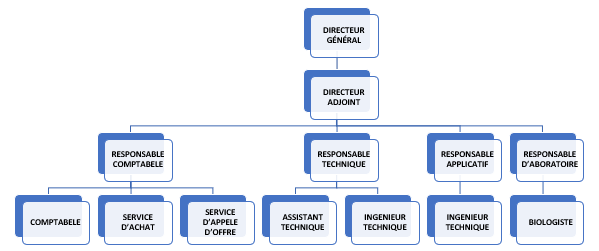
\includegraphics{chapitres/images/postes.PNG}
		\caption{Arborescence des postes dans molbiol-expert}
		\label{fig:labelname}
	\end{figure}

	
	\subsection{\textcolor{green}{Les activités de molbiol-expert :}}
	
	 L'entreprise se spécialise dans l'importation, l'exportation, la distribution et la maintenance de dispositifs médicaux et de réactifs à usage de diagnostic in vitro. Elle propose également l'importation, la distribution et la commercialisation de matériel de laboratoire et médical, ainsi que de fournitures pour les laboratoires d'analyses médicales, comme des matériels, consommables, produits chimiques, produits biologiques et réactifs.\newline
	
	Molbiol-expert offre également des services de conseil, de consultation, d'expertise et d'assistance technique et scientifique réglementaire dans les domaines liés au matériel médical. Elle représente également le service médical d'assistance technique, et réalise des audits et des inspections.\newline
	
	Enfin, l'entreprise est également impliquée dans l'importation, l'exportation, l'achat et la vente ferme ou à la commission de divers produits et articles. Avec son expertise, ses produits et ses services, Molbiol-expert est une entreprise complète dans le domaine médical et de laboratoire, offrant une grande variété de solutions pour les professionnels de ce secteur.\newline
	
	\subsection{\textcolor{green}{Conclusion :}}

	MolbiolExpert est une entreprise spécialisée dans le domaine de la biologie qui propose une large gamme de services de pointe dans les domaines du diagnostic moléculaire, des puces à ADN, du séquençage haut débit, de la chimie, de l'immunoanalyse et de l'anatomie pathologique. L'entreprise a été fondée par des experts universitaires en génétique humaine qui ont travaillé pendant 16 ans dans le secteur des ventes, du marketing et de la gestion des applications pour le diagnostic moléculaire, les puces à ADN et le séquençage haut débit pour le Maghreb. Ils ont également étendu leur expertise dans d'autres domaines de la biologie tels que la chimie, l'immunoanalyse et l'anatomie pathologique. Les partenaires de MolbiolExpert sont des acteurs clés dans le domaine de la biologie moléculaire et du diagnostic, et elles peuvent donc être des partenaires de MolbiolExpert dans différents aspects de son activité, tels que la recherche, la production ou la commercialisation de produits et services.
	
	MolbiolExpert propose des services d'importation, d'exportation, de distribution et de maintenance de dispositifs médicaux et de réactifs à usage de diagnostic in vitro, ainsi que l'importation, la distribution et la commercialisation de matériel de laboratoire et médical. L'entreprise propose également des fournitures pour les laboratoires d'analyses médicales, comme des matériels, consommables, produits chimiques, produits biologiques et réactifs. MolbiolExpert offre également des services de conseil, de consultation, d'expertise et d'assistance technique et scientifique réglementaire dans les domaines liés au matériel médical. Elle représente également le service médical d'assistance technique, et réalise des audits et des inspections.	
	\newpage
\end{flushleft}





